% !TeX program = xelatex
% !BIB program = biber

\documentclass[a4paper, monochrome]{article}

\usepackage{longtable}
\usepackage{array}
\usepackage{placeins}
\usepackage{csquotes}
\usepackage{hyperref}
\usepackage{graphicx}
\usepackage{url}
\usepackage{todonotes}
\usepackage{booktabs}
\usepackage{tablefootnote}
\usepackage{dirtree}
\usepackage{siunitx}
\usepackage{multirow}
\usepackage{tabularx}
\sisetup{output-exponent-marker=\ensuremath{\mathrm{e}}}
\usepackage[ngerman]{babel}
\usepackage[
    backend=biber,
    style=apa,
    autocite=inline,
    mincitenames=1,
    maxcitenames=2
]{biblatex}

\addbibresource{thesis-literature.bib}
\addbibresource{thesis-software.bib}
\addbibresource{thesis-online.bib}

\newcommand{\code}[1]{\texttt{#1}}

\selectlanguage{ngerman}

\def\UrlFont{\rmfamily}

\begin{document}

\begin{titlepage}
    \begin{center}
        \vspace*{1cm}

        \textbf{\Large Bildbasierte Digitalisierung von historischen Toninformationsträgern}

        \vspace{0.5cm}
        Untertitel
                
        \vspace{1.5cm}


        \vfill
                
        Master-Arbeit zur Erlangung des akademischen Grades eines\\
        M.Sc. Digital Humanities

        \vspace{3cm}
                
        Eingereicht von: David Fuhry
        
        \vspace{0.2cm}

        Matrikel-Nr. 3704472\\
        Zschochersche Str. 32\\
        04229 Leipzig

        \vspace{1cm}

        Erstbegutachter: Prof. Dr. Phil. Manuel Burghardt \\
        Zweitbegutachter: N.N.
        
        \vspace{0.2cm}
                    
        Computational Humanities\\
        Institut für Informatik\\
        Universität Leipzig\\
        Augustusplatz 10\\
        04109 Leipzig 
                
    \end{center}
\end{titlepage}

\tableofcontents

\thispagestyle{empty}

\newpage

% Introduction

\pagenumbering{arabic}

\section{Einleitung}

Historische Medien wie Lochplatten und Klavierrollen sind die ältesten, kommerziell in größerer Stückzahl produzierten und auch für den Privatgebrauch gedachten Toninformationsträger.
Sie wurden vom Ende des 19. Jahrhunderts bis zur frühen Mitte des 20. Jahrhunderts von einer Vielzahl von Musikstücken, durch verschiedene Hersteller und in einer hohen Zahl unterschiedlicher Formate produziert.
Die Medien sind zeithistorische Zeugnisse aus einer Zeit, in der privater Musikkonsum erstmals einer breiteren Gruppe von Personen möglich wurde.

Neben durch die Hersteller aus Kompositionen erstellten Medien existieren mit den sogenannte Player Rolls auch Notenrollen, die an einem speziell modifizierten Klavier von kontemporären Pianist:innen eingespielt wurden.
Diese Notenrollen bilden die einzigen Aufnahmen vieler der bekanntesten Pianist:innen aus einer Zeit, in der Audioaufnahmen technisch noch nicht ausgereift genug für die Aufnahme musikalischer Darbietungen waren.

Diese Eigenschaften machen solche historischen Toninformationsträger zu einer wichtigen Ressource für die moderne musikwissenschaftliche Forschung.
Während eine signifikante Anzahl von Medien, insbesondere Notenrollen, bis heute überlebt hat, wird sich ihr Zustand auf absehbare Zeit weiter verschlechtern und so zu irreversiblen Verlusten von Medien und den darauf enthaltenen Informationen führen.

Um diese zeithistorischen Dokumente auch in Zukunft für die musikwissenschaftliche Forschung zugänglich zu und gleichzeitig weitere Schäden an den Medien, etwa durch Abnutzung, zu minimieren bietet sich die Digitalisierung ebendieser an.
Dazu zählt zum einen die Erstellung von hochauflösenden Bildern der Medien, zum anderen aber auch die Digitalisierung der auf den Medien kodierten Toninformationen.
Verfahren zu diesem Zweck existieren, sind aber überwiegend schlecht dokumentiert und der Öffentlichkeit nicht problemlos zugänglich (siehe Abschnitt \ref{Forschungsstand}).

Das Musikinstrumentenmuseum der Universität Leipzig ist im Besitz einer umfangreichen Sammlung von solchen historischen Toninformationsträgern.
Im Rahmen des vergangenen Forschungsprojektes TASTEN wurden von ca. 3000 der Notenrollen aus dieser Sammlung Scans erstellt.

Ziel des aktuellen Forschungsvorhabens DISKOS an der Forschungsstelle des Musikinstrumentenmuseums ist die Digitalisierung dieser Notenrollen und weiterer, plattenförmiger Toninformationsträger aus derselben Sammlung, sowie die inhaltliche Analyse der digitalisierten Medien.
Eine kurze Übersicht dazu findet sich bei \textcite[]{khulusi_2022}.
Zur Umsetzung der Ziele des Forschungsprojektes soll unter anderem eine Anwendung entwickelt werden, die Medien aller Formate in der Sammlung verarbeiten kann.
Die Anwendung soll auch für die inhaltlichen Analysen nutzbar sein.

Zu diesem Zweck wurde die in dieser Arbeit beschriebene Software implementiert.
Sie ist in der Lage, aus den Bilddaten von historischen Toninformationsträgern, die darauf kodierten musikalischen Informationen zu extrahieren.

Es wird zunächst ein voll funktionsfähiges Verfahren zur Digitalisierung von Lochplatten vorgestellt.
Ebenso wird eine erste Implementierung für ein Verfahren zur Digitalisierung von Notenrollen eingeführt.
Die Anwendung gibt nach der Verarbeitung der Bilddaten eine standardisierte Midi-Datei aus.
Im weiteren werden die in die Anwendung integrierten Analyse- und Visualisierungstools, die in Zusammenarbeit mit den am Forschungsprojekt beteiligten Musikwissenschaftler:innen zur Beantwortung musikwissenschaftlicher Fragestellungen entwickelt wurden, demonstriert.



% Historische Toninformationsträger

\FloatBarrier
\section{Historische Toninformationsträger}

\begin{figure*}[t]
    \centering
    
\includegraphics[width=\textwidth]{graphics/placeholder.png}
    \caption{Lochplatten zweier verschiedener Typen aus dem Bestand des Musikinstrumentenmuseums der Universität Leipzig}
    \label{platten}
\end{figure*}

Als Toninformationsträger\footnote{Auch Historical Music Storage Media.} im Sinne dieser Arbeit werden die Medien bezeichnet, die zum Betrieb von mechanischen Musikinstrumenten benötigt werden.
Eine Definition für mechanische Musikinstrumente ist etwa in \textcite[]{mgg_mechanische} gegeben:

\begin{quotation}
    Mechanische Musikinstrumente (selbstspielende Musikinstrumente, Musikautomaten, Automatophone) sind Musikinstrumente, bei denen die Tonfolge selbsttätig durch einen Toninformationsträger gesteuert wird. Die Mehrzahl der mechanischen Musikinstrumente reproduziert Musik ohne Einwirkungsmöglichkeit des Menschen. \parencite[I. Definition]{mgg_mechanische}
\end{quotation}

Die Geschichte solcher mechanischen Musikinstrumente reicht zurück bis in die Antike, in der bereits einfache Orgeln existierten die über das setzen von Stiften auf einer sich drehenden Walze gesteuert werden konnten.
Den Höhepunkt ihrer Popularität erreichten sie während des späten 19. und frühen 20. Jahrhunderts, als eine Vielzahl von verschiedenen, immer komplexeren mechanischen Instrumenten konstruiert wurde \parencite[10-12]{bowers_1972}.
Mit der Entwicklung von besseren und günstigeren Methoden zur Audioaufnahme und -reproduktion in den 1930ern wurden die mechanischen Musikinstrumente praktisch komplett vom Markt verdrängt \parencite[2]{zoltan_1994}.
Für eine ausführliche Übersicht über die Geschichte der mechanischen Musikinstrumente sei auf die entsprechende Literatur verwiesen, etwa \textcite[]{bowers_1972,bowers_1975} sowie \textcite[]{mgg_mechanische}.

Die Medien für solche mechanischen Instrumente kodieren Informationen aus denen das mechanische Instrument Musik erzeugen kann.
Üblicherweise werden dafür zumindest grundlegende Informationen wie der Beginn, die Länge sowie die zugehörige Note für jeden Ton auf dem Medium kodiert.
Es existieren aber auch Instrumente und mit ihnen Formate von Toninformationsträgern die zusätzlich weitere Informationen zu Dynamik und Spielweise kodieren können.
Im weiteren sollen vorrangig die für diese Arbeit relevanten Typen und Formate von Toninformationsträgern weiter betrachtet werden.
% Platten: 1882 bis 1910, Rollen 1900 bis 1930
Diese wurden im Zeitraum zwischen 1882 und 1930 produziert und lassen sich grob in zwei Kategorien unterteilen: Plattenförmige sowie rollenförmige Medien, wobei die plattenförmigen Medien sowohl zeitlich als auch technologisch als Vorgänger der Rollen betrachtet werden können.

\subsection{Plattenförmige Toninformationsträger}

Plattenförmigen Medien wurden ab ca. 1875 produziert und stellten einen paradigmenwechsel in der Konstruktion mechanischer Musikinstrumente dar.
Waren bei früheren Modellen die Toninformationen direkt im Instrument kodiert (beispielsweise über Walzen), wurden sie nun separat auf Platten kodiert und waren somit erstmals unabhängig vom Instrument.
Eine solche Platte hat zumeist eine kurze Laufzeit von einer kleinen einstelligen Zahl von Minuten und konnte damit zumindest kürzere Stücke oder Motive aus größeren Kompositionen enthalten.
Durch diese Entwicklung wurde es erstmals Möglich eine größere Sammlung von Musikstücken zu besitzen \parencite[III.5.c. Plattenspieldosen und Drehinstrumente]{mgg_mechanische}.

Frühe Formate dieser Form von mechanischen Instrumente nutzten Platten aus Pappe auf denen die Toninformationen in Form von Löchern kodiert sind (im Folgenden Lochplatten genannt).
Lochplatten dieser Formate sind sich grundsätzlich recht ähnlich und unterscheiden sich vor allem in den verfügbaren Tönen sowie den physischen Abmessungen der Medien.
Beispiele für zwei Lochplatten unterschiedlicher Formate dieses Typs sind in Abbildung \ref{platten} zu sehen.

Die Lochplatten haben mehrere Spuren, jede Spur ist einem bestimmten Ton zugeordnet, meist sind die Spuren aufsteigend nach Tonhöhe sortiert, mit der tiefsten Note auf der innersten Spur.
Die Töne selbst wurden mittels Löchern binär in die Platten kodiert, dort wo ein Loch vorhanden ist klingt der Ton der entsprechenden Spur.
Wichtig anzumerken ist, dass die meisten Formate nicht chromatisch angelegt waren, die populären Platten der Marke Ariston beispielsweise haben 24 Spuren decken aber über 3 Oktaven ab.\footnote{Siehe \textcite[]{mxp_2003520} für eine genaue Aufschlüsselung des Tonvorrats dieses Formates.}
Durch das auslassen bestimmter Töne ergaben sich zwar Einschränkungen bei der Kodierung von musikalischen Stücken auf die Medien, es konnte aber ein größerer Tonumfang abgebildet werden ohne die Medien und Abspielgeräte in unpraktikable Größen zu skalieren.

\begin{figure*}[t]
    \centering
    
\includegraphics[width=\textwidth]{graphics/placeholder.png}
    \caption{Abspielgerät für Lochplatten der Marke Ariston aus dem Bestand des Musikinstrumentenmuseums der Universität Leipzig}
    \label{aristonplayer}
\end{figure*}

Die Abspielgeräte für solche Platten (siehe Abbildung \ref{aristonplayer}) nutzen Verfahren zur Tonerzeugung, dass dem einer Mundharmonika nicht unähnlich ist.
Eine Lochplatte wurde in ein Abspielgerät eingelegt das über eine Leiste mit Zungen verfügt die den gesamten Radius des informationstragenden Teils der Lochplatte bedeckt.
Zum Abspielen wurde die Lochplatte, je nach Gerät per Handkurbel oder automatisiert, Gedreht und Luft wurde durch die Zungen bewegt.
An den Stellen an denen Löcher vorhanden waren konnte die Luft durch die Zungen passieren, so dass ein Ton erzeugt wurde.
Der so entstehende Klang dieser sogenannten Organetten wurde jedoch häufig als nicht zufriedenstellend empfunden \parencite[III.5.c. Plattenspieldosen und Drehinstrumente]{mgg_mechanische}.

Eine der Entwicklungen die gemacht wurden um dieses Defizit im Klang auszugleichen war der mechanische Klaviervorsetzer.
Dieser nutzt Platten die denen für die Organetten sehr ähnlich sind und Informationen nach dem selben Prinzip kodierten.
Im Gegensatz zu diesen war im Abspielgerät selbst (siehe Abbildung \ref{aristonplayer}) allerdings keine Tonerzeugung integriert.
Stattdessen besaß das Gerät eine Reihe mechanischer Finger, die, vor einem Klavier platziert, das auf der Lochplatte kodierte Stück auf diesem "spielten".

Eine andere Weiterentwicklung der frühen Organetten stellen plattenförmige Medien aus Metall dar.
Bei der Produktion solcher wurden kleine Teile des Blechs umgebogen, so dass Noppen entstanden die in der Lage waren Tonkämme anzureißen.
Die Abspielgeräte für solche Platten verfügten häufig über Zusatzinstrumente wie Triangeln oder Trommeln und waren unter anderem in Wirtshäusern sehr populär \parencite[III.5.c. Plattenspieldosen und Drehinstrumente]{mgg_mechanische}.
Während die Digitalisierung solcher Metallplatten Teil des DISKOS Projektes ist, ist sie aufgrund der fundamental unterschiedlichen Art der Informationskodierung auf diesen Medien kein Teil dieser Arbeit.

Im Rahmen des DISKOS-Projektes wurden Bilder eines vollständiges Konvolut aus 60 Lochplatten der Marke Ariston angefertigt die mit der in dieser Arbeit vorgestellten Software digitalisiert werden.
Weitere 40 Lochplatten für einen Klaviervorsetzer befinden sich noch im Fotografieprozess, konnten aber bereits für Testdigitalisierungen genutzt werden.

\subsection{Notenrollen}

\begin{figure*}[t]
    \centering
    
\includegraphics[width=\textwidth]{graphics/placeholder.png}
    \caption{Abspielgerät für Lochplatten der Marke Ariston aus dem Bestand des Musikinstrumentenmuseums der Universität Leipzig}
    \label{pianoroll}
\end{figure*}

Während die mit der Lochplatte eingeführte Trennung von Abspielgerät und Toninformationen eine signifikante Weiterentwicklung gegenüber den früheren, walzenbasierten mechanischen Musikinstrumenten darstellte, wurde mit der Notenrolle\footnote{Auch Klavierrolle genannt.} ein weiterer Entwicklungsschritt gemacht.
Dieses um die Jahrhundertwende eingeführte Format unterscheidet sich zum einen in der Form der Toninformationsträger, die nun als mehrere Meter lange Rollen ausgeführt wurden, aber vor allem durch die eingesetzten Techniken in den Abspielgeräten.
Ein Abbild einer solchen Rolle ist Abbildung \ref{pianoroll} zu entnehmen.

Die Veränderungen an der Art der Informationskodierung auf den Notenrollen im Vergleich zu Lochplatten ist relativ klein.
Zunächst unterscheiden sich die Notenrollen vor allem durch die neue physische Form die eine Spielzeit von bis zu 15 Minuten ermöglichte.
Eine Notenrolle ist analog zu den früheren Lochplatten in mehrere Spuren unterteilt, die nun allerdings nicht mehr kreisförmig, sondern parallel, meist über die Rollenbreite von Bass (Links) nach Diskant (Rechts) sortiert, angelegt sind.
Die Spuren enthalten weiterhin Löcher die über ihre Position die Toninformationen auf der Notenrolle kodieren.
Ein wesentlicher Unterschied zu Pappplatten besteht in der Kodierung länger zu spielender Töne: Diese werden nun nicht mehr durch eine durchgehende Lochung sondern durch in sehr kurzem Abstand platzierte, z.T. auch überlappende, Löcher kodiert.

Frühe Abspielgeräte funktionierten, analog zu mechanischen Klaviervorsetzern für Pappplatten, als Vorsetzer und unterschieden sich im wesentlichen durch die längere Laufzeit der Notenrollen.
Der entscheidende Vorteil dieses Systems lag in der pneumatischen Steuerung des Abspielgeräts.
Zum Abspielen wird die Rolle in das Abspielgerät eingelegt und dieses erzeugte, bei den ersten Geräten durch menschliche Kraft, später durch Elektromotoren, ein Vakuum über die gesamte Rollenbreite.
Erreichte die Rolle nun eine Stelle an der ein Loch vorhanden war, kann die Luft durch das Loch strömen und so eine pneumatische Steuerung betreiben.
Diese erlaubte es über die Stärke des angelegten Vakuums auch die Stärke des Anschlags auf dem bespielten Klavier zu variieren \parencite[III.5.d. Selbstspielende Klaviere]{mgg_mechanische}.

Mit dieser Technik wurden kurz vor der Jahrhundertwende die ersten selbstspielenden Klaviere\footnote{Auch Player Pianos genannt.} konstruiert.
Die meisten dieser Klaviere verfügten über 2 separate Windladen für die Erzeugung des Vakuums und konnten so die Lautstärke von Bass und Diskant getrennt regulieren.
Während die Variation der Vakuumstärke bei den früheren Modellen, genau wie die Wahl der Geschwindigkeit, noch durch die benutzende Person erfolgte, wurden schnell zunehmend komplexere Abspielgeräte und Rollenformate entwickelt bei denen diese Aufgabe vom Abspielgerät selbst übernommen wurde \parencite[III.5.d. Selbstspielende Klaviere]{mgg_mechanische}.

Im Jahr 1904 patentierte die Firma Welte mit dem Welte-Mignon-System das erste Reproduktionsklavier\footnote{Auch Reproducing Player Piano genannt.} ein System, das komplett ohne menschliche Eingaben Musikstücke wiedergeben konnte \parencite[]{mgg_mechanische}.
Um dies zu ermöglichen wurden Informationen beispielsweise zu Dynamik und Pedalbenutzung auf dafür vorgesehenen Spuren der Notenrolle kodiert.
Die Rollen des Typs Welte-Mignon Welte T100 etwa besaßen 100 Spuren von denen nur 80 zu Tönen zugeordnet waren, die übrigen 20 dienten zur Steuerung des Abspielgerätes \parencite[]{mxp_2002522}.

Solche Informationen konnte im Herstellungsprozess entweder manuell kodiert werden oder aber durch die direkte Aufnahme von Stücken über speziell dafür konstruierte Aufnahmeklaviere erzeugt werden.
An diesen konnten Künstler:innen ein Stück einspielen welches danach in einem mehrstufigen Prozess durch den Rollenhersteller auf eine Notenrolle übertragen wurde.
Das genaue Verfahren mit dem dies Geschah wurde durch die Hersteller mit größter Geheimhaltung geschützt und da keines der Aufnahmegeräte bis heute überdauert hat kann darüber nur spekuliert werden \parencite[]{zoltan_1994}.

Da Audioaufnahmen zur damaligen Zeit noch nicht in vergleichbarer Zeit möglich waren, bescherten grade diese eigens eingespielten Künstlerrollen den Reproduktionsklavieren eine enorme Popularität.
Schnell entwickelte sich eine Vielzahl von verschiedenen Systemen von Reproduktionsklavieren und dazugehörigen Toninformationsträgern und in den 1920er Jahren hatte die Mehrzahl der bekannten Pianist:innen für einen oder mehrere der Hersteller Notenrollen eingespielt \parencite[]{bowers_1972}.

Im Rahmen des vorangegangenen TASTEN-Projekts wurden zwischen 2018 und 2020 am Musikinstrumentenmuseum der Universität Leipzig ca. 5000 Notenrollen in Form von Bildern digitalisiert.
Von diesen liegen ca. 3000 als vollständige Scans vor, von dem restlichen ca. 2000 der Rollen sind nur die Anfänge der Rolle, auf denen Metainformationen wie Titel, Format, etc. vermerkt sind, gescannt worden.
Das gesamte Konvolut umfasst über 30 verschiedene Formate von Notenrollen.
Während im Rahmen des DISKOS-Projektes aus den Scans von Notenrollen aller vorliegenden Formate Midi-Dateien generiert werden sollen, beschränkt sich diese Arbeit auf Rollen des Typs Hupfeld Phonola Solodant, einem verhältnismäßig einfach Format mit 77 Spuren.

% Theorie

\section{Forschungsstand} \label{Forschungsstand}

Das bisherige Forschungsinteresse zur Digtialisierung von historischen Toninformationsträgern konzentriert sich stark auf die Verarbeitung von Notenrollen.
Dies dürfte vor allem auf die Existenz der bereits erwähnten, von kontemporären Pianist:innen eingespielten Notenrollen zurückzuführen sein.
Aber auch die bessere Verfügbarkeit, bedingt durch die hohe produzierte Stückzahl aber auch durch die spätere Produktionszeit und die damit besseren Chancen von heute noch funktionsfähigen Medien, kann ein Faktor sein der zu dieser Diskrepanz am Forschungsinteresse beiträgt.

Die einzigen bekannten Arbeiten zur Digitalisierung von Lochplatten sind im Rahmen des SISAR-Projekts der Italian Mechanical Music Association (AMMI) entstanden \parencite[]{pedrazzini_2013,perretti_2014}.
Im Rahmen dieses Projekts sollen verschieden Typen von historischen Toninformationsträgern digitalisiert werden.
Dabei arbeiten die Autor:innen auch mit Pappplatten des Types Ariston, für die eine Anwendung entwickelt wurde mit der Bilder dieser runden Medien in eine viereckige, einer Notenrolle ähnliche Darstellung transformiert werden können um sie später mit Software zur Digitalisierung von Notenrollen bearbeiten zu können \parencite[]{perretti_2014}.
Eine solche Anwendung wurde ebenfalls im Rahmen des Forschungsprojektes entwickelt \parencite[]{conversion}.
Die Umwandlung in eine Midi-Datei erfolgt dabei mittels hinterlegten Informationen zum Medienformat und den vorhandenen Spuren, das Ausrichten der Spuren auf dem Scan erfolgt manuell.

Leider sind die eingesetzten Methoden praktisch undokumentiert, so dass sich weder zu Qualität und Funktionalität der entstehenden Digitalisate, noch zum aktuellen Entwicklungsstand eine sinnvolle Einschätzung vornehmen lässt.
Auch ist die eingesetzte Software weder als Quellcode noch in binärer Form öffentlich verfügbar, so dass auch auf diesem Weg kein Schluss auf die Güte des Vorgehens möglich ist.

Dennoch können diese Arbeiten zeigen, dass die Digtialisierung von Lochplatten und Notenrollen viele Ähnlichkeiten aufweisen.
Dazu gehören zum einen die ähnliche Art der Informationskodierung (durch Löcher), aber auch viele mechanische Eigenschaften der Abspielgeräte.
Beide Formate wurden durch luftbetriebene Mechanismen von den Abspielgeräten ausgelesen, so dass auch die Art der Informationsdekodierung grundsätzlich ähnlich ist.
Dies legt nah die Digtialisierung der beiden Medienformate als gemeinsamen Themenbereich zu betrachten.
Die vorhandenen Ansätze zur Digitalisierung von Notenrollen können folglich auch als relevant für Verfahren zur Digitalisierung von Lochplatten betrachtet werden.

Die ersten Überlegungen zu solchen Verfahren lassen sich in den 70er Jahren verorten, in den 90ern und frühen 2000ern existierten bereits mehrere Systeme im weiteren Umfeld der digitalen Verarbeitung von Notenrollen \autocite[]{colmenares_2011}.
Allgemein lässt sich feststellen, dass die Projekte aus dieser Zeit überwiegend durch interessierte Privatpersonen und weniger durch akademische Forschung entstanden sind.
Eines der ersten Projekte dieser Art war das \textit{Philips Ampico-Apple} System von Peter Stephens \parencite*[]{stephens}, das die Digitalisierung von Notenrollen des Types Ampico ermöglichte.
Ein späteres Beispiel aus 1996 ist die Entwicklung einer Lösung zur Digitalisierung von Notenrollen mehrerer Formate von Wayne Stahnke \parencite[]{stahnke_1996}.
Als letztes Beispiel dieser privaten Projekte, sei Spencer \textcite[]{chase_2003} genannt, der ebenfalls ein System zur Digitalisierung von Notenrollen konstruierte, aber auch daran interessiert war diese Digitalisate anschließend wieder auf physischen Instrumenten abspielen zu können.
Eine weitere größere Sammlung von digitalisierten Klavierrollen existierte auf der, inzwischen nicht mehr verfügbaren, Website der International Association of Mechanical Music Preservationalists (IAMMP)\footnote{\href{http://www.iammp.org/}{www.iammp.org}}.

Ziel dieser privaten Projekte war es primär die Information auf den Notenrollen zu konservieren und sie auf anderen Geräten wieder abspielbar zu machen.
Gemein haben diese Enthusiasten-Projekte eine sehr beschränkte bis komplett fehlende Dokumentation der Prozesse die zur Digitalisierung genutzt wurden.
Meist wurden die Verfahren entweder entweder gar nicht oder nur auf Mailinglisten oder (inzwischen häufig nicht mehr verfügbaren) privaten Websites dokumentiert.
Die verwendete Software ist häufig proprietär und steht heute nicht mehr für eine Analyse zur Verfügung.
Auch die für die erstellten Digitalisate verwendeten Dateiformate sind insbesondere bei den älteren Projekten proprietär und nur begrenzt dokumentiert.
Bei größeren Sammlungen, wie etwa der der IAMMP, ist eine Nachvollziehbarkeit der Ersteller:innen und der genutzten Methoden der Digitalisate nur eingeschränkt gegeben.
Diese Faktoren schränken die wissenschaftliche Verwendbarkeit der Digitalisierungsprozesse aber auch der erzeugten Digitalisate stark ein.

Eine frühe wissenschaftliche Arbeit zur Digitalisierung von Notenrollen findet sich bei \textcite[]{zoltan_1994}.
Die Autoren beschreiben die Digtialisierung von Notenrollen des Types Welte-Mignon.
Über einen Rollenscanner werden Bilder der Klavierrollen erzeugt aus welchen nach der softwareseitigen Verarbeitung zwei Midi-Dateien generiert werden.
Eine Midi Datei enthält nur die Informationen zu Tonhöhe und Länge, die andere enthält auch die in der Notenrolle kodierten Informationen zu Dynamik ein.
Die Autoren konnten, bedingt durch die verfügbare Technologie, einige Aspekte der Digtialisierung nur bedingt bzw. durch manuelle Korrekturen durchführen, so etwa das Erkennen von Expressionskurven oder der Umgang mit Defekten an der Notenrolle wie Rissen im Papier.
Sie nutzten bereits Techniken die sich in späteren Arbeiten wiederfinden, so wird etwa der Rollenrande dynamisch über den Verlauf der Rolle verfolgt, um durch Deformationen des Papiers entstandene Ungenauigkeiten auszugleichen.

\textcite[]{debrunner_201300} nutzt für die Digitalisierung von Notenrollen des Typs Welte-Philharmonie sowie Welte-Mignon T100 einen Zeilenscanner und eine eigene Software.
Die verwendete Software ist dabei grunsätzlich in der Lage die Digitalisierung in eine Midi-Datei automatisch durchzuführen, benötigt aber bei einem signifikanten Teil der Rollen manuelle Korrekturen.
Das genaue Digitalisierungsverfahren ist nicht dokumentiert, der Schwerpunkt der Arbeit lieft klar auf der Verarbeitung der auf den Notenrollen kodierten Steuerungsinformationen, welche ausführlich dokumentiert werden.

Eine Arbeit die sich spezifisch mit den Herausforderungen der Erzeugung von MIDI Dateien aus bereits digitalisierten, in Matrizenform vorliegenden Klavierrollen beschäftigt findet sich bei \textcite[]{colmenares_2011}.
Die Autor:innen nutzen dabei Digitalisate die mit der Technologie von \textcite[]{stahnke_1996} erzeugt wurden.
Im Gegensatz zu dessen proprietärer Digitalisierungstechnologie setzen die Autor:innen aber einen Schwerpunkt darauf  ihren Umwandlungsprozess ausführlich zu dokumentieren.

Sie gehen dabei sowohl allgemein auf das Dekodierverfahren für Klavierrollen in Matrizenform ein als auch insbesondere auf die Umsetzung der Kontrollspuren ins Midi Format.
Von interesse ist insbesondere das von den Autoren zur Validierung ihrer Ergebnisse eingesetzte Verfahren.
Sie führen dabei einen Wellenformvergleich von, aus den von ihnen erzeugten Midi-Dateien generierten, Audio Dateien mit den von \textcite[]{stahnke_1996} selbst erzeugten und vertriebenen Audio-CDs der gleichen Notenrollen durch \parencite[70ff]{colmenares_2011}.
Dabei können sie die Genauigkeit ihres Verfahrens demonstrieren, das bis auf kleinere Abweichungen authentische Ergebnisse produziert.
Problematisch scheint allerdings, dass die Genauigkeit dieser Validierungsmethode stark von der Genauigkeit der ursprünglichen, von \textcite[]{stahnke_1996} mittels eines prorietären, nicht öffentlich dokumentierten Prozesses durchgeführten, Digitalisierung abhängig ist.

Das aktuellste und umfangreichste Vorhaben zur Digitalisierung von Notenrollen ist das Player Piano Projekt an der Stanford University.
Dieses wurde 2014 ins Leben gerufen um die umfangreiche Sammlung von Notenrollen in der eigenen Bibliothek Forscher:innen und anderen interessierten zugänglich zu machen \autocite[]{shi_2019}.
Aktuell befinden sich circa 20.000 Notenrollen in der Sammlung in Stanford von denen ca. 1000 erfolgreich digitalisiert wurden \autocite[]{broadwell_2022}.
Das Projekt fokussierte sich dabei zunächst auf die Digitalisierung von Notenrollen des Typs Welte-Mignon T-100, umfasst inzwischen aber auch die Digitalisierung Rollen anderer Formate.

Dafür wurde zunächst ein Gerät konstruiert, dass es erlaubt hochauflösende\footnote{TIFF mit 300dpi Auflösung.} Bilder der Notenrollen anzufertigen.
Teil des Scanprozesses ist dabei das anwenden verschiedener, automatischer Fehlerkorrekturen für physische Defekte der gescannten Notenrolle.
So wird etwa, ähnlich zu \textcite[]{zoltan_1994} ein Korrekturverfahren zur Begradigung der Notenrolle genutzt, mit dem, besonders in den späteteren Teilen der Rollen auftretende, Verzerrungen kompensiert werden können.
Weiterhin setzten die Autor:innen Filter ein um Löcher die uncharakteristisch Merkmale aufweisen\footnote{Beispielsweise bei Form oder Orientierung des Lochs.} und vermutlich auf Beschädigungen zurückzuführen sind zu erkennen.
Schnell aufeinanderfolgende Löcher, die von Originalabspielgeräten als einzelne Note gespielt werden\footnote{Sogenannte \textit{Bridges}.}, werden zusammengefasst \autocite[519-520]{shi_2019}.

Auch die Funktionalität der Steuerungsspuren wird in dem von \textcite[521-522]{shi_2019} vorgestellten Digitalisierungsverfahren möglichst originalgetreu in den erzeugten Midi-Dateien abgebildet.
Ebenso werden weitere Anpassungen vorgenommen um das Abspielverhalten auf Originalabspielgeräten zu simulieren, wie etwa die leichte Temposteigerung die durch die sich verändernden Rollendurchmesser beim Abspielen einer Notenrolle vermutet wird.
Aus den generierten Midi-Dateien wird mittels eines generischen Software-Pianos eine Audiodatei generiert.no gerendert wurden.

Aktuell arbeiten die Autor:innen unter anderem am Pianolatron, einer webbasierten Softwarelösung die Notenrollen darstellen und interaktiv abspielen kann \parencite[]{vijoy_2022}.
Die Software erlaubt es dabei eine Notenrolle aus dem Bestand von ca. 1000 digitalisierten Rollen abzuspielen, Parameter wie Abspielgeschwindigkeit und Lautstärke können interaktiv angepasst werden.
Auch können verschiedene Parameter der Emulation der mechanischen Komponenten der Originalabspielgeräte angepasst werden, so dass sich, in Fällen in denen durch Verlust der Originalabspielgeräte keine notwendigerweise originalgetreue Abbildung möglich ist, diese sich experimentell Testen lassen.
Es bestehen weitere Interaktionsmöglichkeiten, so können Nutzer:innen etwa durch Auswählen von auf den Rollen vorhandenen und durch die Software erkannten Noten weiter Informationen zu diesen einsehen.
Insgesamt bildet das Pianolatron schon jetzt eine umfangreiche und vielversprechende Abspiel- und Visualsierungsumgebung für Notenrollen.



% Vorgehen

\FloatBarrier

\section{Softwarebasierte Digitalisierung von historischen Toninformationsträgern}

\subsection{Das \code{musicbox} Paket}

\begin{figure*}[t]
    \centering
    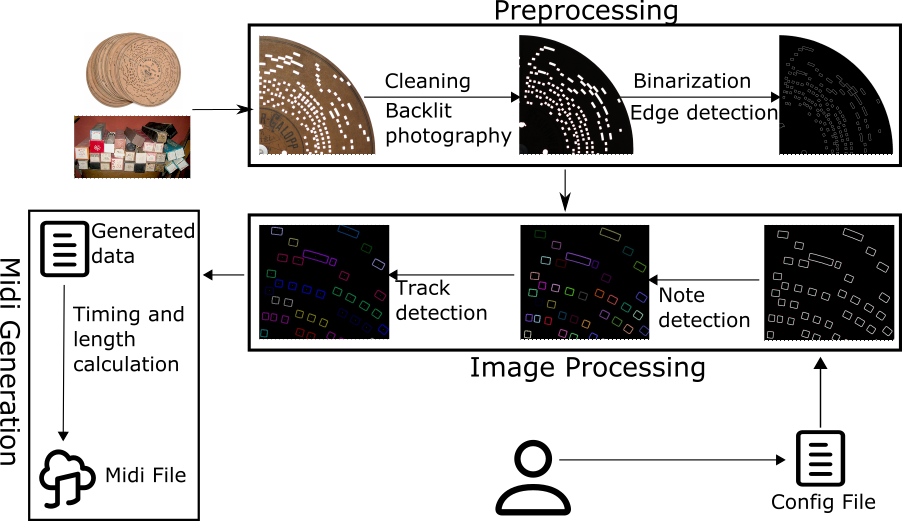
\includegraphics[width=\textwidth]{graphics/flow_diagram.png}
    \caption{Übersicht über den Digitalisierungsprozess einer Lochplatte mit der \code{musicbox} Software.}
    \label{softwareworkflow}
\end{figure*}

Im Rahmen des DISKOS-Projektes soll eine einheitliche Softwarelösung für die Generierung von Midi-Dateien aus Bildern der Toninformationsträger im Bestand des Musikinstrumentenmuseums der Universität Leipzig erstellt werden.
Zu diesem Zweck wurde die, dieser Arbeit zugrundeliegende, Software in Form des \code{musicbox} Paketes in der Programmiersprache Python \parencite[]{van1995python} implementiert.
Diese Software ermöglicht es den gesamten Umwandlungsprozess von der Vorverarbeitung der Bilddaten bis zur Erstellung der Midi-Datei automatisiert vorzunehmen.
Es werden während der Verarbeitung idealerweise keine externen Eingaben benötigt.

Um die für die Verarbeitung der diversen unterschiedlichen Formate von Toninformationsträgern notwendige Flexibilität zu ermöglichen und gleichzeitig eine möglichst hohe Wiederverwendbarkeit der einzelnen Bestandteile zu gewährleisten, ist die Software modular aufgebaut und durch Konfigurationsdateien flexibel anpassbar.
Mit diesem Ansatz soll in der Zukunft für die Verarbeitung eines neuen Formats von Toninformationsträgern idealerweise die Erstellung einer Pipeline aus einzelnen Verarbeitungsschritten und die Angabe von Formatspezifischen Informationen wie Spurenbelegung, Abmessungen etc. ausreichen.

Diese Funktionalität wird über Profile, die in einer YAML-Konfigurationsdatei hinterlegt sind, realisiert.
In dieser wird für ein Profil zunächst eine Pipeline bestehend aus mehreren Verarbeitungsschritten definiert.
Die verfügbaren Verarbeitungsschritte sind innerhalb des Paketes in mehreren Python-Dateien nach dem Teilgebiet des Umwandlungsprozesses zu dem sie gehören aufgeteilt.
Der Name des Verarbeitungsschrittes setzt sich dabei aus Datei und Methodennamen zusammen, z.B. \code{preprocessing.binarization}.
Neben der Verarbeitungspipeline werden die für den Umwandlungsprozess benötigten Parameter in der Konfigurationsdatei abgelegt.
Diese beinhalten Metadaten zum Format des Mediums das verarbeitet werden soll, etwa die Anzahl und die Belegung der vorhandenen Spuren, aber auch Parameter für die Vorverarbeitung der Bilddaten, etwa den Threshold für die Bildbinarisierung.

Die Software ist dabei auf einfache Erweiterbarkeit ausgelegt.
Neue Verarbeitungsschritte können als Methode in der entsprechenden Python-Datei definiert werden und werden dann, wenn sie Bestandteil einer Verarbeitungspipeline sind, automatisch zur Laufzeit aufgerufen.
Zusätzlich können in einer separaten Konfigurationsdatei Metainformationen zum Verarbeitungsschritt definiert werden.
In dieser Datei werden Informationen zu den für den Verarbeitungsschritt erforderlichen Parametern, sowie aus anderen Verarbeitungsschritten benötigten bzw. für diese bereitgestellten Daten gespeichert.
Diese Informationen nutzt die Software, um vor der Ausführung einer Verarbeitungspipeline zu prüfen, ob diese ausführbar ist und ob alle benötigten Parameter im Konfigurationsprofil definiert sind.

Der Umwandlungsprozess selbst kann entweder über das Einbinden des Paketes in ein eigenes Python-Skript oder über ein bereitgestelltes Wrapper-Skript angestoßen werden.
In Abbildung \ref*{softwareworkflow} ist eine grobe Übersicht über den allgemeinen Umwandlungsprozess zu sehen.

Grundlegend gilt es im Umwandlungsprozess von Lochplatten und Notenrollen die Informationen über Tonhöhe, -anfang und -länge zu finden.
Dazu müssen zunächst die einzelnen Löcher auf dem Medium identifizieren werden.
Für jedes dieser Löcher sind im Folgenden der Start- und Endpunkt der Lochung auf dem Medium zu identifiziert, aus welchen Tonanfang und -länge abzuleiten sind.
Abschließend muss jedes Loch noch der entsprechenden Spur auf dem Medium zugeordnet werden, um die Tonhöhe bestimmen zu können.

Ziel der Umwandlung ist in jedem Fall die Erstellung einer Midi-Datei.
Eine solche speichert keine Audioinformationen, sondern, nicht unähnlich der ursprünglichen Toninformationsträger, Informationen wann welcher Ton für wie lange klingt.
Midi-Dateien können als etablierter Standard für die Speicherung solcher Informationen betrachtet werden und sind das Umwandlungsziel oder -zwischenziel bei allen aktuelleren Verfahren zum Digitalisieren von Toninformationsträgern, siehe etwa \textcite[65]{colmenares_2011} oder \textcite[518]{shi_2019}.

Im Folgenden wird dieser Umwandlungsprozess anhand einer voll funktionalen Pipeline für die Umwandlung von Lochplatten, sowie einer sich noch im Prototypstadium befindlichen Pipeline für Notenrollen genauer erläutert.

\subsection{Digitalisierung von Pappplatten}

\begin{figure*}[t]
    \centering
    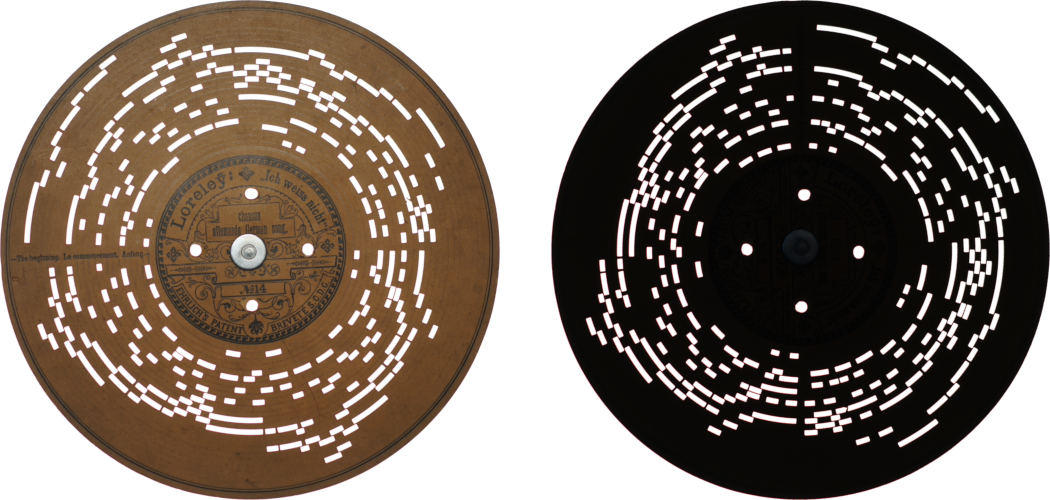
\includegraphics[width=\textwidth]{graphics/ariston_pictures.png}
    \caption{Zur Dokumentation angefertigtes Bild einer Lochplatte sowie das für die Digitalisierung bestimmte Bild der gleichen Lochplatte.}
    \label{pappplattenphotos}
\end{figure*}

Lochplatten sind die ältesten Toninformationsträger, die im Rahmen des DISKOS-Projekts digitalisiert werden sollen.
Die Verarbeitung der Lochplatten ist durch die runde Form etwas komplexer als die von Notenrollen.
Gleichzeitig sind die auf den Medien kodierten Toninformationen vergleichsweise simpel, es sind keine Steuerungsinformationen oder ähnliches vorhanden.
Auch reduziert die relativ kleine Größe der Medien die rechnerische Komplexität des Unwandlungsprozesses im Vergleich zu Notenrollen.\footnote{Vorliegende Notenrollenscans erreichen bei 300 DPI Dateigrößen bis zu 5GB.}
Sie wurden deshalb als erstes Format für die Umwandlung in Midi-Dateien ausgewählt.

Der Digitalisierungsprozess beginnt mit der Begutachtung der Medien durch am Projekt beteiligte Musikwissenschaftler:innen, die die Medien reinigen, auf Schäden untersuchen und anschließend alle auf dem Medium selbst vorhandenen Metainformationen, zusammen mit allen gefundenen Beschädigungen des Mediums, dokumentieren.
Anschließend wird eine hochauflösende Fotografie des Mediums angefertigt.
Die Lochplatten werden dazu in einer, speziell für diesen Zweck konstruierten, Aufhängung platziert, in welcher sie mit Hintergrundbeleuchtung fotografiert werden können.
Abbildung \ref{pappplattenphotos} zeigt beispielhaft das Bild einer Lochplatte der Marke Ariston, sowohl als normales Foto als auch als Bild für die weitere digitale Verarbeitung.

Die Bilder, die für die softwarebasierte Verarbeitung vorgesehen sind, unterscheiden sich dabei von denen, die zur Dokumentation und Konservierung angefertigt werden.
Während die Platten für die normalen Fotografien nach der Plattenbeschriftung ausgerichtet werden, werden die Lochplatten für die weitere Digitalisierung mit der Startmarkierung der Lochplatte auf 0 Grad ausgerichtet.
Dadurch entfällt die Notwendigkeit die Startmarkierung softwareseitig zu identifizieren.
Auch werden diese Aufnahmen mit veränderten Belichtungseinstellungen vorgenommen, um einen höheren Kontrast zwischen den Löchern auf der Platte und der Platte selbst zu erreichen.\footnote{Während der anfänglichen Entwicklung der hier vorgestellten Software wurden für die Verarbeitung Bilder ohne diese Einstellungen oder Hintergrundbeleuchtung erfolgreich verwendet. Es ist davon auszugehen, dass sich solche Bilder mit leichten Anpassungen der Vorverarbeitung problemlos verwenden lassen.}

Die vorliegenden Bilddaten werden für die weitere Verarbeitung grundsätzlich als Graustufenbild eingelesen.
Im Anschluss wird zunächst eine einfache, threshold-basierte Binarisierung angewendet.
Für diesen, sowie die meisten weiteren bildbasierten Verarbeitungsschritte, wird die OpenCV \parencite[]{opencv_library} Bibliothek im Zusammenspiel mit Numpy \parencite[]{harris2020array} genutzt.
Der genutzte untere Threshold für die Binarisierung (60) wurde experimentell ermittelt, um eine möglichst optimale Erhaltung der Strukturen der Platten, bei gleichzeitiger Minimierung von Artefakten zu gewährleisten.

Im nächsten Schritt wird ein Kantenerkennungsalgorithmus auf das Bild angewendet.
In früheren Versionen der Software wurde hierfür der Canny-Algorithmus eingesetzt \parencite[]{canny_1986}.
Dies führte mitunter zu Problemen, da die Abstände zwischen einzelnen Löchern auf den Pappplatten in Extremfällen nur einzelne Pixel betragen und die mit dem Canny-Algorithmus berechneten Kanten sich in solchen Fällen überlappen können.
Um dieses Problem zu umgehen wird ein morphologischer Kantenerkennungsalgorithmus eingesetzt, der zunächst mit einem 3x3 Kernel eine Erosion des Bildes durchführt und anschließend aus der Differenz des Originalbildes und der Erosion die Kanten bildet.
Dieses Verfahren stellt sicher, dass die Kanten immer auf der Innenseite der Löcher der Lochplatten liegen.

\begin{figure*}[t]
    \centering
    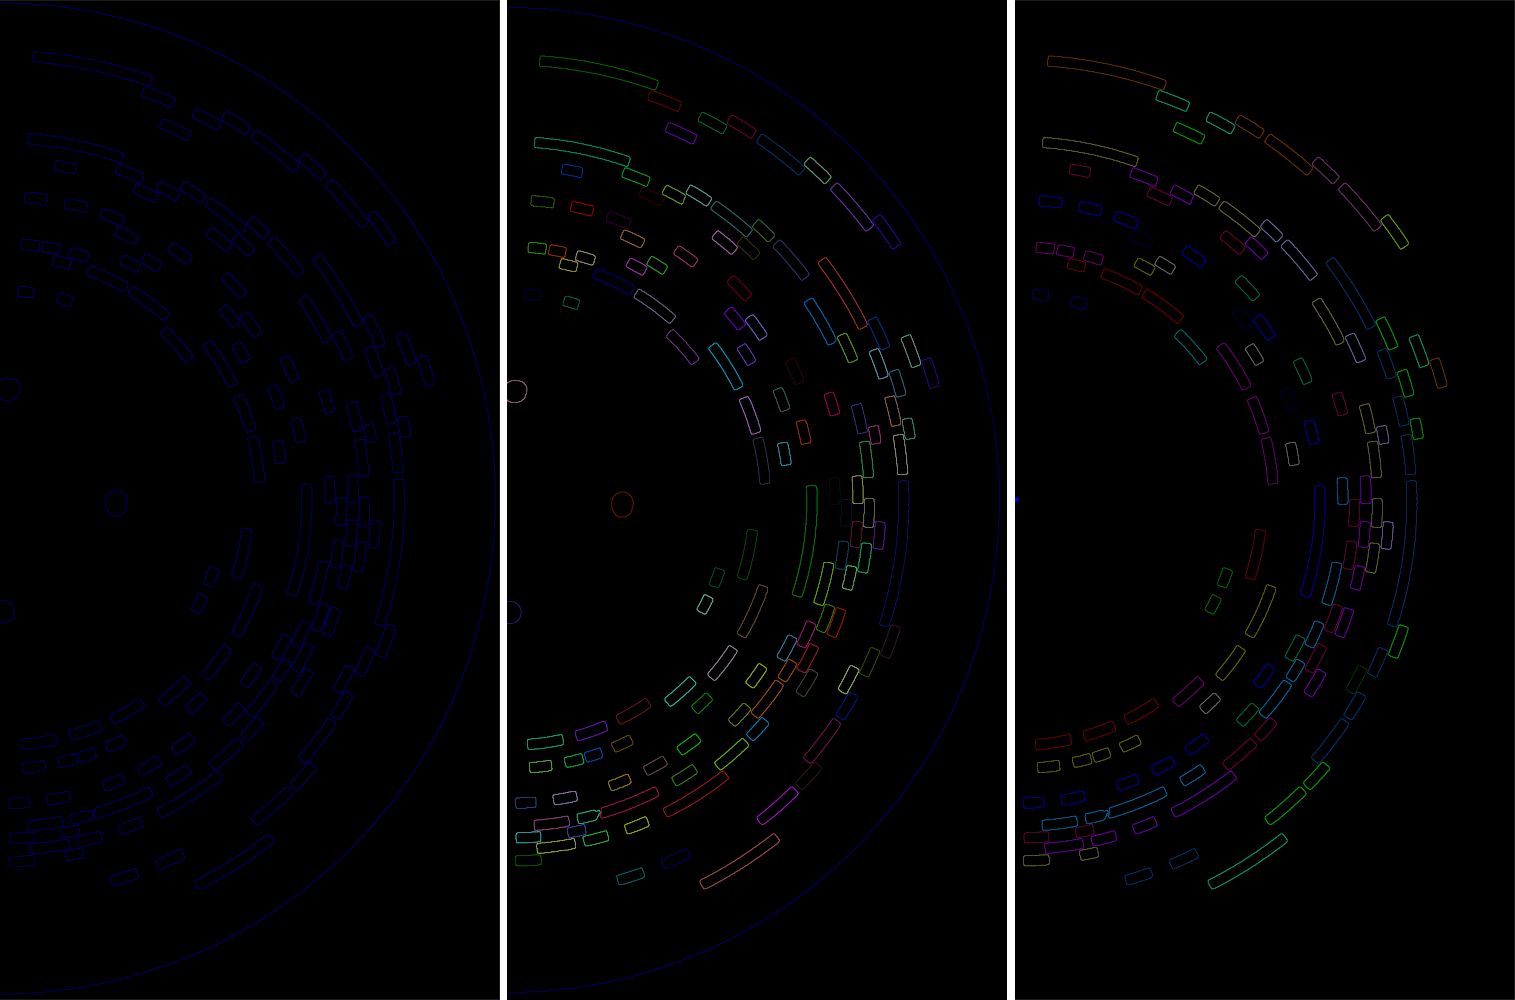
\includegraphics[width=\textwidth]{graphics/processing.png}
    \caption{Bild einer Ariston Lochplatte nach der Kantenerkennung, dem Identifizieren von Löchern sowie der Zuordnung der Löcher zu Spuren.}
    \label{pipelinesteps}
\end{figure*}

Um das nun vorliegende Bild der Kanten weiter zu Zerlegen und Komponenten wie die einzelnen Notenlöcher identifizieren zu können, wird im weiteren ein Algorithmus zum Finden von 2-verbundenen Komponenten aus Scikit-Image \parencite[]{scikit-image} eingesetzt.
Die so gefundenen Komponenten werden für die weitere Verarbeitung in jeweils ein Array mit den Koordinaten der zugehörigen Pixel umgewandelt, um Berechnungen von Distanzen etc. zu vereinfachen.
Aus diesen Komponenten wird die äußere Kante der Platte identifiziert (die größte zusammenhängende Komponente), sowie rechnerisch, mithilfe von in der Konfiguration hinterlegten Messungen, die innere Grenze des mit Tonspuren belegten Bereichs bestimmt.
Es werden alle gefundenen Komponenten die innerhalb dieser inneren Begrenzung oder außerhalb des äußeren Plattenrandes liegen herausgefiltert, da diese keine Tonlöcher sein können und somit für die weitere Verarbeitung uninteressant sind.

Alle verbleibenden Komponenten sind die Kanten von Löchern auf der Lochplatte.
Einzelne Platten weisen Beschädigungen in der Form von Einrissen zwischen zwei Löchern auf, die dazu führen können, dass diese Löcher als eine gemeinsame Komponente und damit im Weiteren als ein Einzelner, über die gesamte Länge der beiden Löcher klingender, Ton interpretiert werden.
Dies entspricht allerdings auch dem Verhalten eines Originalabspielgerät beim Abspielen einer Platte mit solchen Beschädigungen, so sie denn in einem insgesamt noch spielbereiten Zustand ist.
Um zu gewährleisten, dass das Digitalisat dem tatsächlich vorliegenden Medium so ähnlich wie möglich ist, findet deshalb keine Korrektur solcher Einrisse statt.

Im nächsten Schritt wird der Mittelpunkt der Lochplatte bestimmt.
Da die Lochplatten beim Fotografieren an dem Loch in ihrer Mitte aufgehängt werden, ist dieses auf den Bildern nicht identifizierbar.
Zur Mittelpunkbestimmung wird deshalb ein rechnerisches Verfahren angewendet.
Es wird mittels des Algorithmus von \textcite[]{halir1998numerically} eine Ellipse auf die Punkte des äußeren Plattenrandes regressiert und anschließend aus der Ellipsengleichung der Mittelpunkt bestimmt.
Dieses Verfahren liefert grundsätzlich sehr akkurate Ergebnisse, hat jedoch bei einzelnen Lochplatten mit bestimmten Deformationen Probleme.
Dort wird zwar der korrekte Mittelpunkt des äußeren Plattenrandes identifiziert, dieser ist aber nicht der Mittelpunkt der Tonspuren auf der Platte.
In diesen Fällen ist aktuell eine manuelle Korrektur des Mittelpunkts nötig.

Anschließend werden die einzelnen erkannten Löcher ihren entsprechenden Spuren zugeordnet, so dass die jeweiligen Tonhöhen bestimmt werden können.
Dafür wird zunächst die Distanz, vom Zentroid ausgehend, jeder Komponente zum äußeren Rand sowie zum Mittelpunkt der Lochplatte berechnet.
Aus diesen Distanzen wird die relative Position der Komponente zwischen dem Plattenmittelpunk und dem Plattenrand abgeleitet.
Dies dient zur Reduzierung des Einflusses von Deformationen der Lochplatte auf den Spurzuordnungsprozess.
Anhand dieser Positionen werden die Komponenten in die einzelnen Spuren gruppiert, wozu das MeanShift Clusteringverfahren \parencite[]{meanshift} in der Implementierung in Scikit-Learn \parencite[]{scikit-learn} eingesetzt wird.
Dieses Verfahren wurde gewählt, da es gegenüber den meisten Algorithmen, die spezifisch für das Gruppieren von eindimensionalen Daten entwickelt wurde, den Vorteil bietet kein a priori Wissen über die Anzahl der Cluster zu benötigen.
Da nicht notwendigerweise alle Spuren, die ein Format bietet bei jeder Platte des Formats genutzt werden, ist nur die obere Schranke der Zahl der Cluster bekannt, nicht aber die Zahl der tatsächlich vorhandenen.

Dies beeinflusst auch die Zuordnung der in dem Format existierenden Spuren, zu denen auf dem spezifischen Medium gefundenen.
Um für das Vorhandensein leerer Spuren zwischen den gefundenen Spuren zu kompensieren, wird die durchschnittliche Distanz der gefundenen Spuren zu den jeweiligen Nachbarn berechnet und jeweils zwischen die Spuren mit der höchsten Distanz eine leere Spur eingefügt.
Dies wird wiederholt, bis die Zahl der vorhandenen Spuren der der in dem Format existierenden Spuren entspricht.
Ist dieser Schritt abgeschlossen sind die gefundenen Löcher ihren Spuren zugeordnet und die mit ihnen verbundene Tonhöhe ist ermittelt.

Um die nun noch fehlenden Informationen zu Tonanfang und -länge zu finden, wird für jedes Loch das minimal umschließende Rechteck berechnet.
Anhand dessen wird je ein Punkt am, im Sinne der Abspielrichtung der Lochplatte, Anfang und Ende des Lochs bestimmt.
Für beide Punkte wird dann, ausgehend vom Plattenmittelpunkt, der Winkel zwischen Punkt und dem Rollenanfang berechnet.
Der kleinere Winkel ist der Tonanfang, der Zeitpunkt an dem die Note zu klingen beginnt, die Differenz der beiden Winkel die Tonlänge, die Zeit für die der Ton klingt.

Die Originalabspielgeräte für diese Medien spielen Töne leicht verzögert zum Erreichen des Loches ab.
Dies ist in der Bauweise begründet, erst wenn eine bestimmte Menge Luft durch ein Ventil strömt entsteht ein hörbarer Ton, üblicherweise wenn etwa die Hälfte eines Ventils frei liegt.
Ein ähnliches Verhalten ist auch beim Schließen der Ventile am Lochende zu beobachten.
Aktuell findet hierfür keine Anpassung statt, dies wäre aber in der Zukunft über Konfigurationsparameter vorstellbar.

Weiterhin ist anzumerken, dass die berechneten Angaben zu Timing und Tonlänge in Grad vorliegen und nicht in Schlägen, wie sie in Midi-Dateien kodiert sind.
Während softwareseitig Methoden bereitgestellt werden um diese Angaben um einen festen Faktor zu skalieren, ist eine genaue Bestimmung des Zeitmaßes nicht zuletzt dadurch erschwert, dass es sich bei den Originalabspielgeräten um handbetriebene Automaten handelte.
Das Tempo war deshalb abhängig von der Drehgeschwindigkeit der Kurbel und somit variabel.
Eine bessere Bestimmung des Zeitmaßes würde vermutlich durch die Bestimmung von Takt- und Schlaglänge des Stückes auf dem Medium möglich, die aber nicht zum aktuellen Funktionsumfang der Software gehört.

Aus den bis hier gewonnen Informationen wird abschließend mittels der MIDIUtil Bibliothek \parencite[]{midiutil} eine Midi-Datei erstellt, die die auf dem Toninformationsträger kodierten Informationen enthält.
Diese Dateien können anschließend beliebig weiterverwendet werden.
Eine Überführung in eine Auralisierung, in Form einer Audiodatei, kann entweder über generische Softwareinstrumente erfolgen oder z.B. über die, sich ebenfalls am Musikinstrumentenmuseum in Entwicklung befindliche, midiAuralizer \parencite[]{midiauralizer} Software.
Diese ermöglicht es beliebige Midi-Dateien mittels, im Rahmen des DISKOS-Projekts aufgenommener, Tonvorräte von historischen Instrumenten, darunter auch Originalabspielgeräte für Lochplatten des Typs Ariston, zu Audiodateien umzuwandeln.

Das hier vorgestellte Verfahren wurde in dieser Form für die Umwandlung des gesamten Konvolutes der Lochplatten des Types Ariston verwendet.
Ebenso konnte es in testweisen Digitalisierungsversuchen mit Lochplatten für einen mechanischen Klaviervorsteller ähnlich gute Ergebnisse erzeugen.
Die nötigen Anpassungen beschränken sich dabei auf die Erstellung eines neuen Konfigurationspresets mit Informationen zu den Abmessungen und Spuren des neuen Formats.

\subsection{Digitalisierung von Klavierrollen}

Als nächster Schritt der Entwicklung der vorgestellten Softwarelösung wurde ein vergleichsweise simples Format von Notenrollen für die Digitalisierung ausgewählt, Notenrollen der Marke Hupfeld Phonola Solodant.
Notenrollen dieses Formats besitzen 77 Spuren, von denen 73 Spuren Tönen zugeordnet sind, 2 zur Dynamiksteuerung verwendet werden und 2 freibleiben.

Während das vorgestellte Digitalisierungsverfahren für Lochplatten als voll funktionsfähig angesehen werden kann, befindet sich die Lösung für die Umwandlung von Notenrollen noch in einem früheren Entwicklungsstadium und sollte als Prototyp verstanden werden.
So werden die auf den Rollen vorhandenen Steuerspuren zwar korrekt ausgelesen, aber bei der Generierung der MIDI-Dateien aktuell nicht genutzt.
Auch können, zum Teil auf den Rollen abgedruckte, Dynamiklinien durch das Verfahren aktuell nicht ausgewertet werden.
Dennoch stellt das Verfahren in seinem aktuellen Zustand eine grundlegend funktionsfähige Digitalisierunglösung für Notenrollen dar.
Auch zeigt sich im Hinblick auf die Umsetzung des Verfahrens der Vorteil einer modularen Softwarelösung wie der hier vorliegenden.
Während viele Komponenten speziell für die Verarbeitung von Notenrollen implementiert wurden, konnte ein Teil der Komponenten aus dem bereits vorgestellten Prozess wiederverwendet werden.

Die, währen des vorangegangenen TASTEN-Projekts in Zusammenarbeit mit einem externen Dienstleister erstellten, vollständigen Scans von Notenrollen liegen als TIFF-Dateien mit einer Auflösung von 300 DPI vor und bilden die gesamte Notenrolle inklusive Anfang und Ende ab.
Diese Scans wurden, im Gegensatz zu den im Rahmen des DISKOS-Projektes erzeugten Aufnahmen von Lochplatten, vor schwarzem Hintergrund ohne Hintergrundbeleuchtung erstellt.
Aus technischen Gründen umfassen die Scans, je nach Rollenlänge, auch einen längeren, leeren Bereich nach dem Ende der Rolle.

Nach der Binarisierung der Bilder, die mit der gleichen Komponente wie die der Lochplatten erfolgt, wird daher zunächst die Rolle auf die Länge des tatsächlich gelochten Teils gekürzt.
Um diesen Bereich zu identifizieren, wird über die gesamte Länge des Scans für jede Zeile der relative Anteil der Pixel mit Inhalt errechnet.
Anschließend wird bestimmt in welchen Zeilen der Anteil der gefüllten Pixel über 80\% liegt\footnote{Die Scans der Notenrollen weisen einen, je nach Format, unterschiedlich großen Rand neben der Rolle auf. 80\% wurde experimentell als sinnvolle untere Schranke bestimmt.} und aus diesen die längste zusammenhängende Folge von Zeilen ausgewählt.
Diese Methode schließt, je nach konkret betrachtetem Scan, einen gewissen Teil von Rollenanfang und -ende mit ein, dies erwies sich jedoch in der Praxis als unproblematisch für die weitere Verarbeitung.

Die folgenden Schritte des Findens von zusammenhängenden Komponenten sowie das Umwandeln dieser in Koordinatenlisten geschehen mit den gleichen Verfahren, die auch für Lochplatten genutzt wurden.
Um die Ränder der Rolle zu identifizieren, werden über die gesamte Länge der Rolle 100 zufällige Zeilen ausgewählt und die in diesen Zeilen liegenden verbundenen Komponenten gezählt.
Die beiden Komponenten die in den meisten, praktisch sogar allen, Zeilen vorkommen sind die Kanten an den Rändern der Rolle.

Aufgrund der unterschiedlichen Aufnahmetechnik der Notenrollen, gegenüber den später aufgenommenen Platten, weisen sie nach der Binarisierung und Kantenerkennung deutlich mehr Artefakte auf.
Um dies zu kompensieren, werden im nächsten Schritt Filter auf die gefundenen Komponenten angewendet.
Zum einen wird für jede verbundene Komponente ermittelt, ob sie aus mehr oder weniger Pixeln besteht als der über die Pixelzahl aller verbundenen Komponenten, mit Ausnahme der Rollenränder, gebildete Mittelwert.
Alle Komponenten, die aus weniger Pixeln bestehen als die durchschnittliche Komponente werden entfernt.
Die verbleibenden Komponenten werden noch einmal über ihre Form gefiltert.
Es wird geprüft ob das gerundete Verhältnis von Höhe zu Breite der Komponente im Intervall $[1,2]$ liegt.
Während ein rundes Loch in einer Notenrolle üblicherweise etwa genau so breit wie hoch sein sollte, kann es bei sehr eng platzierten Löchern dazu kommen, dass diese als eine gemeinsame Komponente erkannt werden.
Deshalb werden solche Komponenten, die bis etwa doppelt so hoch wie breit sind, nicht entfernt.
Abgesehen von einzelnen Verarbeitungsfehlern sind alle noch verbleibenden Komponenten die Kanten von Löchern auf der Notenrolle.

Anschließend werden die Informationen zu den auf der Rolle kodierten Noten extrahiert.
Zu diesem Zweck wurde im Rahmen des DISKOS-Projekts von Musikwissenschaftler:innen der Gleitbock des Abspielgerätes\footnote{Die Komponente auf der die Notenrolle aufliegt und an der das Vakuum anliegt das für die Tonerzeugung nötig ist.} vermessen und die genauen Maße, sowie der assoziierte Ton für jede Spur dokumentiert, siehe \textcite[]{mxp_2002548}.
Mit diesen Informationen kann, durch einfaches Berechnen der relativen Distanzen zwischen jedem Loch und den Rollenrändern, die zugehörige Spur für jedes Loch ermittelt werden.
Da Notenrollen sich, bedingt durch die lange Zeit der Lagerung, insbesondere im späteren Verlauf der Rolle verziehen können, wird die Rolle für diese Berechnungen in Segmente zu jeweils mindestens 1000 Pixeln unterteilt und die Positionsbestimmung für jedes Segment separat vorgenommen.
Die Segmente werden dabei so gewählt, dass kein Loch geteilt wird.
Sollte der Bedarf bestehen können diese Segmente auch kleiner gewählt werden, die gewählte Größe hat sich jedoch bis jetzt als ausreichend erwiesen, um, zumindest leichte, Deformationen der Rolle ausgleichen zu können.
Gleichzeitig sollte diese Größe noch ausreichend groß sein, um zu verhindern, dass kürze Einriss der Rolle oder ähnliche Beschädigungen die Spurbestimmung negativ beeinflussen.
Tonanfang und -länger werden durch die Position des höchsten und tiefsten Punkts einer Komponente bestimmt.

Im Gegensatz zu den Abspielgeräten für Lochplatten wurden Reproduktionsklaviere meist von elektrischen Motoren betrieben und erlaubten so eine präzise Einstellung der Abspielgeschwindigkeit.
Die vorgesehene Abspielgeschwindigkeit war bei einigen Formaten auf dem Rollenanfang, in der Einheit feet per 10 Minutes vermerkt \parencite[63]{colmenares_2011}.
Da die Scanauflösung bekannt ist, kann der Umrechnungsfaktor Pixel per Second ($pps$) aus den feet per minute ($fpm$) wie in Gleichung \ref{eq:1} errechnet werden.
Werden die vorher ermittelten Timings und Tonlängen nun mit diesem Faktor skaliert, liegen die Tonlängen in Sekunden vor.
Zeitangaben in MIDI-Dateien erfolgen grundsätzlich als Schläge (Beats) und nicht in Sekunden, \footnote{Alternativ ist es auch möglich die Zeitangaben in Ticks zu hinterlegen, diese stehen allerdings in einem direkten Verhältnis zu Schlägen.} weshalb zusätzlich die Geschwindigkeit der erzeugten Midi-Datei auf 60 BPM festgelegt wird.
Mittels dieser Skalierung sollten die Digitalisate der Notenrollen mit vorhandenen Tempoangaben annähernd im Originaltempo abgespielt werden.

\begin{equation} \label{eq:1}
    pps = \frac{fpm * 12 * 300}{60}
\end{equation}

Aufgrund der mechanischen Eigenschaften der Pneumatik der Originalabspielgeräte wurden Löcher, die einen sehr kleinen Abstand zueinander hatten wie ein durchgehendes Loch abgespielt.
Die praktische Grenze dieses Verhaltens ist nicht klar bekannt und dürfte zwischen Geräten variieren.
\textcite[7]{zoltan_1994} gibt sie mit 10-12 Wiederholungen die Sekunde an, die noch als einzelne Töne interpretiert werden sollten
Darauf basierend wird eine obere Grenze von 12 Noten die Sekunde als differenzierbar wiedergebbar angenommen.
Alle Noten, die so eng beieinanderliegen, dass sie diese Grenze überschreiten, werden durch die Software zusammengefasst.

Abschließend wird analog zur Verarbeitung der Lochplatten eine Midi-Datei generiert.
Das hier vorgestellte Verfahren wurde u.a. zur Umwandlung einer Skalenrolle\footnote{Eine Klavierrolle die aufsteigend alle Spuren mehrmals abspielt und ursprünglich zum Testen und Kalibrieren der Abspielgeräte genutzt wurde.} genutzt und konnte dort zufriedenstellende Ergebnisse produzieren.


% Umsetzung

\FloatBarrier
\section{Analysetools und Visualisierungen}

Neben der Umwandlung der historischen Toninformationsträger in Midi-Dateien steht die Nutzbarmachung der generierten Daten für die Musikwissenschaftliche Forschung im Fokus dis DISKOS-Projekts.
Zu diesem Zweck implementiert das \code{musicbox} Paket Funktionen zur Erstellung von Analysedaten und Visualisierungen aus den verarbeiteten Bildern.
Diese Funktionen werden in Zusammenarbeit mit den am Forschungsprojekt beteiligten Musikwissenschaftler:innen entwickelt und orientieren sich an den Fragestellungen die diese an die Toninformationsträger haben.
Während im weiteren Verlauf des DISKOS-Projekts insbesondere die Erkennung von Mustern in den Aufnahmen sowie vergleichende Analysen vorgenommen werden sollen, fokussierte sich die bisherige. hier vorgestellte Arbeit vor allem auf grundlegendere Methoden zur besseren Erschließung der vorliegenden Daten.

Eine erste Frage die die Musikwissenschaftler:innen an die Medien hatten war die Identifizierung von Akkorden, also gemeinsam klingenden Tönen, auf den Medien.
Zu diesem Zweck sind im Softwarepaket mehrere Methoden implementiert.
So lassen sich zum einen die klingenden Akkorde von den Basstönen\footnote{Die im Akkord meist den Grundton bilden.} aus untersuchen.
Dabei werden alle Basstöne, die Grenze bis zu der ein Ton als Basston angesehen wird ist frei konfigurierbar, ausgewählt und für jeden dieser Töne alle anderen gleichzeitig klingenden Töne ermittelt.
Eine weitere Methode durchsucht das Medium sequentiell und ermittelt für jeden Ton die anderen gleichzeitig klingenden Töne.
Beide Methoden lassen sich flexibel konfigurieren um beispielsweise festzulegen ob auch Töne mit eingeschlossen werden sollen, die bereits vor der betrachteten Note angespielt wurden, aber noch klingen während diese angespielt wird.
Die Ergebnisse werden anschließend in Textform ausgegeben und sind für die Analyse verfügbar.

\begin{figure*}[t]
    \centering
    
\includegraphics[width=\textwidth]{graphics/placeholder.png}
    \caption{Keys go here}
    \label{keys}
\end{figure*}

Insbesondere der letzte hörbare Akkord ist dabei für die musikwissenschaftliche Analyse von Interesse, da er üblicherweise direkte Rückschlüsse auf die Tonart des Stückes ermöglicht.
Für die Tonartbestimmung eines Stückes existieren weiterhin auch algorithmische Ansätze, wie etwa das probabilistische Modell von \textcite[]{temperley_2002}.
Die \code{musicbox} Software nutzt die Implementierung dieses Verfahrens im Python Paket music21 \parencite[]{music21} um die Tonart der Stücke auf den bearbeiteten Medien zu bestimmen.
In Abbildung \ref{keys} sind die ermittelten Tonarten für das gesamte vorhandene Konvolut von Platten des Typs Ariston zu sehen.
Die dort sichtbare Dominanz von Stücken in A-Dur im Konvolut legt den Schluss nahe, dass das Format besonders für Stücke in dieser Tonart geeignet war.
Ob dies in dem Tonvorrat den dieses Format enthält begründet liegt oder ob es sich um gesellschaftliche Gründe, wie etwa eine besonders gute Resonanz der Konsumenten auf Stücke in dieser Tonart, eventuell auch spezifisch bezogen auf Stücke die in Form solcher Toninformationsträger vertrieben wurden, handelt ist dabei eine Frage die im weiteren Lauf der musikwissenschaftliche Forschung beantwortet werden muss.

\begin{figure*}[t]
    \centering
    
\includegraphics[width=\textwidth]{graphics/placeholder.png}
    \caption{Barcharts go here}
    \label{barcharts}
\end{figure*}

Neben solchen Analyseverfahren waren die beteiligten Musikwissenschaftler:innen auch an Visualisierungen zur besseren Erschließung der Medien interessiert.
Ein erster Schritt dazu ist die nach der Häufigkeit der einzelnen auf den Medien vorkommenden Tönen.
Zu diesem Zweck wurde eine Funktion implementiert, die die Notenhäufigkeit über das gesamte Medium ermittelt und als Balkendiagramm ausgibt (siehe Abbildung \ref{barcharts}).
Dabei werden durch die Software mehrere Diagramme generiert.

Zunächst wird die Häufigkeit aller Einzeltöne dargestellt, wobei die X-Achse bewusst chromatisch angeordnet ist und auch Töne einschließt die auf dem spezifischen Medium bzw. dem Medienformat insgesamt nicht vorhanden sind.
Dies dient der einfacheren optischen Erkennung von Mustern.
Ein ähnlicher Graph wird auch mit der Summe der Tonlänge pro Ton statt der Vorkommenshäufigkeit erstellt.
Um eine generalisierte Betrachtung zuzulassen werden beide Diagramme auch in einer Form erzeugt, in der die Töne auf ihre Grundtöne reduziert werden, was einen einfachere Betrachtung der Tonhäufigkeiten etwa für Rückschlüsse auf die vorkommende Tonart ermöglicht.
Zur Diagrammerstellung kommt allgemein die Python Bibliothek \code{matplotlib} \parencite[]{Hunter_2007} zum Einsatz.

\begin{figure*}[t]
    \centering
    
\includegraphics[width=\textwidth]{graphics/placeholder.png}
    \caption{Streamcharts}
    \label{streamcharts}
\end{figure*}

Die beteiligten Musikwissenschaftler:innen waren weiterhin an einer Darstellung interessiert die auch die zeitliche Komponente der Medien mit einschließt.
Hierfür wurde ein Streamgraph als Darstellungsform gewählt, der die Häufigkeit der einzelnen Grundtöne über den zeitlichen Verlauf des Mediums anzeigt.
Für die in Abbildung \ref{streamcharts} zu sehende Visualisierung mehrerer Lochplatten wurden für die vorkommenden Noten ein Binning über die zeitliche Komponente des Mediums in 12 Segmente vorgenommen.
Ferner wurden die vorkommenden Töne auf ihre Grundtöne reduziert und diese chromatisch sortiert.
So wird es ermöglicht das Musikstück auf Trends und Veränderungen in seinem zeitlichen Verlauf zu untersuchen.

Diese Streamgraph-Darstellungen haben sich auch als eine praktische Möglichkeit erwiesen eine Form von Fingerprints für einzelne Medien zu erstellen.
In Abbildung \ref{streamcharts} sind die Streamgraphen für 4 verschieden Lochplatten des Typs Ariston zu sehen.
Abgebildet sind jeweils 2 Medien von 2 unterschiedliche Musikstücken, zu denen im Bestand des Musikinstrumentenmuseums mehrere verschiedene Lochplatten vorhanden sind.
Die Lochplatten (1) und (2) enthalten beide Fassungen des Stückes \textit{An der schönen blauen Donau}, Lochplatten (3) und (4) Fassungen des \textit{Schatz-Waltzers}.
Während zwischen Lochplatten (1) und (2) leichte Unterschiede ersichtlich sind, wie etwa die Häufigkeit der Töne B und Cis, sind sich die beiden Diagramme doch strukturell sehr ähnlich, was Tonhäufigkeit und deren Entwicklung über den Verlauf der Platte betrifft.
Demgegenüber lassen Lochplatten (3) und (4) zwar noch Ähnlichkeiten erkennen, etwa der Starke anstieg an vorhandenen Tönen im letzten Abschnitt der Platte, unterscheiden sich allerdings über den gesamten Verlauf verhältnismäßig stark
Dies legt den Schluss nahe, dass Lochplatten (1) und (2) das gleiche Stück beinhalten, während es sich bei den Platten (3) und (4) potentiell um unterschiedliche Arrangements des gleichen Stückes handelt.

Neben den vorgestellten Analysemöglichkeiten erzeugt die Software während der Verarbeitung der Medien auch Reihe von Informationen die die Ergebnisse einzelner Zwischenschritte der Verarbeitung repräsentieren, etwa bildliche und textliche Daten zu gefundenen zusammenhängenden Komponenten und Noten.
Auch diese Daten lassen sich potentiell nutzen um die verarbeiteten Medien zu analysieren.
Mit tabellarischen Daten zu den erkannten Noten lassen sich beispielsweise statistische Betrachtungen der Notenlänge über verschiedene Medien realisieren.

Ebenso lassen sich durch die auf einfache Erweiterbarkeit ausgelegte Architektur der Anwendung neue Analyseschritte problemlos umsetzten und die Methoden haben nicht nur Zugriff auf die final erzeugten Midi-Daten sondern auch auf alle Daten die in Zwischenschritten erzeugt wurden.

% Ergebnisse

\section{Diskussion}

Die in dieser Arbeit vorgestellte Software ermöglicht die automatische Erzeugung von Midi Dateien aus Scans historischer Toninformationsträger.
Sie ist in der Lage als Lochplatten ausgeführte Toninformationsträger aus Pappe nur mit einem hochauflösenden Bild und einigen von Experten dokumentierten Metainformationen zum Format zu verarbeiten.
Die Funktionalität der Anwendung für diesen Zweck ist durch die praktisch vollständige Digitalisierung des Konvoluts von Lochplatten des Typs Ariston im Bestand des Musikinstrumentenmuseums demonstriert.

Auch konnte demonstriert werden, wie die modularität der vorgestellten Software dazu beiträgt andere Formate historischer Toninformationsträger zu verarbeiten.
Unter Wiederverwendung mehrerer Komponenten aus der Verarbeitung der Lochplatten wurde eine frühe Lösung zur digitalisierung von Notenrollen des Typs Phonola Solodant gezeigt.
Die praktikabilität dieser Herangehensweise bestätigt sich durch die erfolgreiche Digitalisierung u.a. einer Skalenrolle dieses Formats. 

Die in der Anwendung integrierten Analysemöglichkeiten können in ihrer aktuellen Form zur Beantwortung grundlegender Musikwissenschaftlicher Fragestellungen, wie etwa das ermitteln der Tonart eines Stückes, beitragen.
Aber auch für weitergehende Untersuchungen wie der Vergleich von mehreren Medien des gleichen musikalischen Stückes werden Funktionen in der Form von Visualisierungen angeboten.

Im Vergleich mit der in \textcite[]{perretti_2014} erwähnten Anwendung zur Digitalisierung von Lochplatten ist vor allem hervorzuheben, dass die hier vorgestellte Anwendung, neben dem erstmaligen erstellen einer Konfigurationsdatei für das Format, keine weitere Eingabe bei der Umwandlung benötigt und diese automatisch vornimmt.
Eine komperative Betrachtung der Digitalisierungsqualität zwischen beiden Anwendungen ist hingegen nicht möglich, da die von \textcite[]{perretti_2014} genutzte Anwendung weder öffentlich zugänglich noch in dem für einen Vergleich nötigen Maß dokumentiert ist.
Aus denselben Gründen ist auch ein Vergleich des Verfahrens zur Digitalisierung von Notenrollen mit bereits existierenden Verfahren nur bedingt möglich.
Sicher kann davon ausgegangen werden, dass alle Verfahren die die auf Notenrollen vorhandenen Steuerungsspuren auswerten und korrekt umsetzten, darunter die von \textcite[]{shi_2019, zoltan_1994, colmenares_2011} vorgestellten, originalgetreuere Ergebnisse liefern als es das hier vorgestellte Verfahren aktuell tut.

Ein wesentlicher Vorteil der hier vorgestellen Anwendung liegt, grade im Vergleich mit den meisten bekannten Verfahren, in der Konzipierung als offene, flexibel erweiterbare Anwendung.
Sie kann so zum einen von allen Interessierten genutzt und angepasst werden, zum anderen sind die genutzten Verfahren so für alle Nutzer:innen nachvollziehbar.

Die in der Anwendung vorhandenen Analysewerkzeuge sind aktuell in Umfang und Tiefe noch nicht vergleichbar mit denen von spezieller Software für diesen Anwendungszweck wie etwa \textit{music21} \parencite[]{music21}.
Im Gegensatz zu diesen bietet sie aber die Möglichkeit Analysen direkt auf den bei der Digitalisierung erzeugten Daten auszuführen und nicht erst auf der abschließend erzeugten Midi-Datei.
Auch die direkte Erzeugung von Visualisierungen aus den vorhandenen Daten unterscheidet sie von üblichen Softwarelösungen für computergestützte Musikanalysen. % Wirklich?!

Während die Digitalisierung neben einem einmaligen Erstellen von Konfigurationsdaten für ein Format keine weiteren Informationen benötigt, ist es wünschenswert die Zahl der erforderlichen Parameter in Zukunft weiter zu reduzieren.
So sollte es etwa möglich sein den optimalen Threshold für die anfängliche Binarisierung der Bilddaten automatisch statt experimentell zu ermitteln.
Dies würde auch die Verarbeitung von mit anderen Aufnahmemethoden als der im Musikinstrumentenmuseum genutzten erstellten Bilder vereinfachen.

Auch die noch sich noch im Prototypstadium befindliche Verarbeitung von Notenrollen soll in Zukunft weiter verbessert werden.
Insbesondere die Emulation des Abspielverhaltens der Originalabspielgeräte steht hier im Mittelpunkt.
Dazu gehören etwa die korrekte Verarbeitung von Steuerungsspuren auf den Medien, sowie das automatische auslesen von auf einigen Medien vorhandenen Dynamikspuren.
Auch andere Gerätespezifische Verhalten, wie etwa eine vermutete Änderung des Abspieltempos durch den sich beim Abspielen verändernden Umfang der auf- bzw. abgerollten Rolle sollen in Zukunft abgebildet werden.

Die in der Software integrierten Analysetools beschränken sich aktuell auf eher grundlegende Analyseschritte und sollen in Zukunft durch weitere Komponenten erweitert werden.
Dazu zählen Verfahren zum Erkennen von Mustern in verarbeiteten Medien, aber auch insbesondere Tools die den Vergleich zwischen Medien ermöglichen.
Verfahren zum Vergleich von Stücken die auf historischen Toninformationsträgern und in einer anderen Form, wie etwa als Notenblatt, vorliegen sowie für Vergleiche über ganze Korpora von digitalisierten Toninformationsträgern stehen dabei im Fokus. 

Schlussendlich sind auch Verfahren zur Validierung der erzeugten Musikdaten wünschenswert.
Während die Ergebnisse der Software aktuell vor allem qualitativ durch Musikwissenschaftler:innen begutachtet werden, sind hier auch Methoden des quantitativen Vergleichs wünschenswert.
Denkbar wäre etwa ein, ähnlich dem von \textcite[]{colmenares_2011} genutzten Verfahren, Vergleich von Wellenformen zwischen mithilfe von Tonvorräten der Originalinstrumenten erstellter, digitalisierter Fassung und Originalaufnahmen.

% Fazit

\section{Fazit}

Historische Toninformationsträger in Form von u.a. Lochplatten und Notenrollen stellen wertvolle, zeithistorische Zeugnisse aus einer Zeit in der privater Musikkonsum erstmals möglich wurde dar.
Im Rahmen der Forschung am Musikinstrumentenmuseum der Universität Leipzig sollen diese Medien präserviert und für die musikwissenschaftliche Forschung geöffnet werden.
Dazu gehört die softwarebasierte Erzeugung von Midi-Dateien aus Bildaufnahmen der Originalmedien.
Auch sollen verschiedene Analyse- und Visualsierungtools geschaffen werden die zur Beantwortung musikwissenschaftlicher Fragestellungen an die Medien beitragen können.

In dieser Arbeit wurde die Implementierung einer Anwendung zu diesem Zweck in Form der Python Software \code{musicbox} vorgestellt.
Es wurde ein Verfahren eingeführt mit dem diese Anwendung aus Lochplatten erfolgreich und vollständig digitale Midi-Dateien erzeugen kann.
Weiterhin wurde ein grundlegendes Verfahren zur Digitalisierung von Notenrollen vorgestellt, welches in seinen Grundfunktionen bereits für die Digitalisierung einzelner Medien nutzbar ist.
Abschließend wurden erste, in der Anwendung integrierte, Analyse- und Visualsierungstools beschrieben, die zur Beantwortung musikwissenschaftlicher Fragestellungen an den Medienbestand genutzt werden können.

Insgesamt konnte ein erfolgreiches Verfahren für die Digitalisierung historischer Toninformationsträger gezeigt werden.
Die dabei entstandene Softwareanwendung bietet durch ihre auf einfache Erweiterbarkeit ausgelegte Architektur eine solide Grundlage für die Verarbeitung weiterer Medienformate sowie die Umsetzung zusätzlicher Visualisierungs- und Analyseverfahren.
In der Zukunft ist die Erweiterung der Anwendung für diese Zwecke geplant.

\clearpage

%
% ---- Bibliography ----
%
%
\setcounter{biburllcpenalty}{7000}
\setcounter{biburlucpenalty}{8000}

\selectlanguage{german}

\printbibliography[title=Literatur, keyword=literature]
\printbibliography[title=Software, keyword=software]
\printbibliography[title=Online, keyword=online]

\clearpage

% Die eidesstattliche Erklärung mit Unterschrift
\textbf{Erklärung der Urheberschaft}

\vspace{1cm}

Hiermit erkläre ich, daß ich die vorliegende Arbeit
selbstständig angefertigt, nicht anderweitig zu Prüfungszwecken vorgelegt und
keine anderen als die angegebenen Hilfsmittel verwendet habe. Sämtliche 
wissentlich verwendete Textausschnitte, Zitate oder Inhalte anderer Verfasser 
wurden ausdrücklich als solche gekennzeichnet.

\vfill

\hspace{2cm} \textbf{Leipzig, 13.08.2021} \hspace{2cm} %
\includegraphics[scale=0.3]{graphics/signature.png}


\vspace{1cm}

\hspace{2cm} Ort, Datum \hfill Unterschrift \hspace{2cm}


\end{document}
